% RMIT University School of CS&IT
% Minor thesis template
% S.M.M. (Saied) Tahaghoghi, 2004
\documentclass[11pt,twoside]{report}
\usepackage{a4wide,caption,epsfig,fancyheadings,url}
\usepackage[colorlinks,citecolor=blue,urlcolor=blue,bookmarks=false,hypertexnames=true]{hyperref}
\usepackage{float}
\usepackage{capt-of}
\usepackage{amsmath}

% Place the correct values here
%Set to the original submission date when submitted amended thesis
\newcommand{\SubmissionDate}{\today}
\newcommand{\student}{Qi Xiong}
\newcommand{\supervisor}{Hai Dong}
\newcommand{\topic}{Enhance the performance of Github repository recommendation by using a Knowledge Graph Neural Network based approach}
\newcommand{\school}{School of Computer Science and Information Technology}
\newcommand{\program}{Masters of Applied Science (Information Technology)}
\newcommand{\institution}{Royal Melbourne Institute of Technology}

% Use the remark command to highlight text for discussion
\newcommand{\remark}[1]{{\bf \em [\marginpar{$\Leftarrow$}#1]}}

\renewcommand{\leftmark}{\student}
\renewcommand{\rightmark}{\topic}
\renewcommand{\headrulewidth}{0pt}
\setlength{\parindent}{0pt}
\setlength{\parskip}{1.5ex plus 0.3ex}

% This is the line spacing - set to 2 for draft submission to
% supervisor, 1.3 for the final submission
\renewcommand{\baselinestretch}{1.00}

\renewcommand{\captionfont}{\it}
\raggedbottom
\graphicspath{ {./Figs/} }

%For Natbib Author, year citation format
% - the opening bracket symbol, default = (
% - the closing bracket symbol, default = )
% - the punctuation between multiple citations, default = ;
% - the letter n for numerical style, or s for numerical superscript
%   style, any other letter for author year, default = author year;
% - the punctuation that comes between the author names and the year
% - the punctuation that comes between years or numbers when common author lists are suppressed (default = ,);
% \bibpunct{[}{]}{;}{a}{,}{;}


\begin{document}

\title{{\Large\bf \topic}}
\author{
A minor thesis submitted in partial fulfilment of the requirements for the degree of
\\\program\\*[10mm]
%\epsfig{figure=Figs/rmit-coa.epsf,width=5cm}
\\\student
\\\school
\\Science, Engineering, and Technology Portfolio,
\\\institution
\\Melbourne, Victoria, Australia
}
\maketitle
\thispagestyle{empty}

\chapter*{Declaration}

This thesis contains work that has not been submitted previously, in
whole or in part, for any other academic award and is solely my
original research, except where acknowledged.

This work has been carried out since July 2021, under the
supervision of {\supervisor}.

\paragraph{}
\vspace{5cm}\noindent \\\student \\
\school\\
\institution\\
\SubmissionDate

\pagenumbering{roman}

\chapter*{Acknowledgements}

I would like to acknowledge and express my warmest thanks to my supervisor Hai Dong for his patience and support. His support on computing resources helped me overcome the obstacle in which my laptop is too old and slow for doing the research. His valuable guidance and advice carried me through the writing of the thesis.

I would also like to extend my thanks to the GH Archive project for open sourcing their dataset of the public GitHub activities of developers and repositories. The dataset provides the most similar use cases in real situations and is ideal for the research of recommending projects.

I would also like to extend my thanks to my fellow students for share their ideas, suggestions and experiences in doing minor thesis projects.

Finally, I thank my families and friends for their continuous help and supports.

{
    \hypersetup{linkcolor=black}
    \tableofcontents
    \listoffigures
    \listoftables
}

\pagenumbering{arabic}

\chapter{Introduction}
\section{background}
GitHub \footnote{https://github.com} is an open-source community that enables developers to manage their repositories via a version control system named Git \footnote{https://git-scm.com/}. Developers can also share their projects and contribute to other developers’ projects in this community.

The recommender system for GitHub repositories is important. Developers tend to find repositories that are similar to the ones they are working on to find functions or ideas which can be reused. Although the search engine provided by GitHub can help find similar repositories, it is always not accurate because it only uses the title of repositories rather than the whole details according to \cite{xu_repersp_2017}. While recommender systems can recommend the most relevant repositories to users based on the preference of users and repositories.

\textit{Most recommender systems have data sparsity and cold start issues.} Due to the long tail effect, few popular products have the most ratings while lots of others have fewer ratings. As a result, the constructed user-item matrix is sparse. It is inefficient for a model to deal with a sparse matrix. If a user does not rate any items then it is hard for the recommender system to recommend items to that user. This is the cold start issue. Because in the beginning, there are always few ratings. Researchers have proposed various approaches to tackle these issues.

One of the approaches is to take the side information which was investigated by \cite{jonschkowski_patterns_2016} of users and items into consideration. Side information can be efficiently integrated into a knowledge graph neural network. With more information that can be used to determine a user's preference, a recommender system thus can fight for data sparsity issues and improve performance. The improvements are promising according to \cite{zhang_knowledge_2020} which applied side information and knowledge graph neural network in mobile APP recommendations.

Many existing works have proposed various GitHub recommender systems. \textit{But none of them can deal with the cold start problem because they ignored the use of the side information for the recommender system.}

This thesis proposed a knowledge graph neural network (KGNN) based model to recommend Github repositories to developers. The performance and the ability to fight data sparsity issues are promising compared with traditional recommender systems. The project of this thesis was open sourced on GitHub \footnote{https://github.com/qinqin65/GitHub-Repo-RS}.

\section{Motivation}
\textit{There is no research in applying KGNN in recommending GitHub repositories while KGNN has the potential to bypass the data sparsity and cold start issues} \cite{mansur_review_nodate}. The recent studies on the GitHub repositories recommender system are based on traditional approaches such as collaborative filtering that are prone to suffer from data sparsity and cold start issues. \textit{For solving those issues, this thesis explores the idea of using the KGNN to recommend GitHub repositories.}

\textit{There is various side information that can be used to build the KGNN based GitHub repositories recommender system.} Users’ behaviours such as "star", "pull" and "clone" can be regarded as side information that indicates users are interested in some repositories. Repositories' programming language can also be considered as side information that guides the recommender system to recommend the repository to the user with the same programming language preference. Those side information can help the KGNN model to achieve the expected outcome.

\section{Research questions}
This research aims to propose a recommender system for GitHub repositories with high performance and the ability to solve data sparsity and cold start issues.

Based on this aim, there are three research questions as list below.

\begin{enumerate}
    \item RQ1: What side information can be used to build a KGNN based repositories recommender system?
    \item RQ2: What’s the performance can the KGNN based repositories recommender system achieve?
    \item RQ3: How better can the KGNN based repositories recommender system mitigate the data sparsity issue?
\end{enumerate}

\chapter{Literature review}
\section{Recommender systems}
According to \cite{mansur_review_nodate, park_literature_2012}, current recommendation approaches can be classified into three categories: collaborative filtering (CF), content based recommendation, hybrid recommendation. CF can be further classified into memory based and model based approaches. Memory based CF does all calculations in the memory. If it calculates the similarities (i.e., similar in preferences) between users and recommends a user's liked items to his or her similar users who do not know the item, Then it is a user based CF. If it calculates the similarities (i.e., similar in descriptions) between items and recommends an item to users who liked its' similar items, then it is an item based CF. Model based CF recommends items by designing a model which takes users and items as inputs. The model often projects users and items into the same latent space in which similar users and items are close to each other. The output layer of the model often reconstruct the relationship between users and items from the latent space and make predictions on the ratings for unknown user-item pairs. Content filtering calculates the similarities (i.e., similar in contents) between items and recommending an item to a user who liked its' similar items. The hybrid recommendation is a combination of those recommendation approaches.

\section{Graph neural networks}
Graph neural network (GNN) was proposed by \cite{gori_new_2005, scarselli_graph_2009} to learn patterns from graph data that traditional machine learning models cannot handle. The idea is aggregating the state (i.e., a state can be the data represented by a node) of neighbour nodes for each node in the graph using an aggregating function. The aggregating function is restricted to be a contraction mapping for the state of each node. Based on the Banach theorem, the output of the aggregating function is unique regardless of the aggregating order. The state is then inputted to an output function to produce an output. The aggregating function and output function can be neural networks. Based on these ideas, the patterns can be distilled from graph data no matter what order and structure the graph changes. GNN has many successful applications such as learning molecular fingerprints \cite{duvenaud_convolutional_2015}.

The applications of GNN in recommender systems have demonstrated great success as well. Because the data in a recommender system can be represented as a graph structure and GNN are very good at handling connections between nodes according to \cite{wu_graph_2020}. Especially in social recommendations, users and their friends can form a graph. Users’ interaction with items can also form a graph. Fan et al. came up with an approach named “GraphRec” which is based on this fact \cite{fan_graph_2019} and proved that the harness of the relationship between user and user, user and item plays an important role in improving the performance of the recommender system. A session that contains a series of events of interaction between a user and items can also be presented in a GNN model and make predictions about the next event such as which item the user will most likely click. This is classified as a session-based recommendation and plays an important role in web services according to \cite{xu_graph_2019}. The GC-SAN model which makes use of the self-attention algorithm was proposed to identify the transitions of nearby items in a session \cite{xu_graph_2019}.

Most GNN models use low dimensional embedding to represent node features to make them more efficient. However, they still need to iterate all nodes in a graph to learn embeddings. It makes the GNN model very hard to scale to a large data set. Hamilton \cite{hamilton_inductive_2018} proposed the GraphSage model to solve this problem by uniformly sampling neighbour nodes and thus reduce the number of nodes to calculate \cite{hamilton_inductive_2018}. Also, GraphSage can be applied to inductive learning such as predicting embeddings for future unseen nodes.

The use of GNN in recommendation can be classified as the general recommendation and sequential recommendation \cite{wu_graph_2020}. The general recommendation can be powered by Knowledge Graph.

\section{Knowledge graph neural networks}
Knowledge Graph neural network is a class of GNN and has gained focus in the field of recommender systems. The side information can be presented as a knowledge graph and can be integrated into a Graph neural network to learn additional knowledge and the performance can be improved accordingly. Zhang et al. \cite{zhang_knowledge_2020} proposed a knowledge graph based approach to recommend mobile Apps and shows promising improvements in performance.

Traditional recommender systems have problems of cold start and data sparsity \cite{mansur_review_nodate, wu_graph_2020, zhang_knowledge_2020} which makes recommendation much difficult in the beginning. Some researchers make use of the side information to help the recommender system to make decisions to solve this problem. The more side information is used the more accurate the recommender system can achieve. There are various types of side information such as the high order relations of items (connect items with two or more linked attributes) \cite{wang_kgat_2019} and semantic information of user-item interactions \cite{wang_knowledge_2019} was explored by researchers. They all show a promising performance according to their papers.

According to \cite{guo_survey_2020}, knowledge graph based recommender systems can be classified into three categories which are embedding-based, connection-based and propagation-based. The embedding-based approach projects the nodes and edges of a graph into a lower dimension space in which linked nodes are close to each other. This approach can scale to a large graph but it cannot capture the connection pattern between nodes. The connection-based approaches mine the pattern of connections in a graph. This approach can use the pattern of connections of a graph to guide the recommendation but paths of the connections need to be specified manually. The propagation-based approach combines the advantages of embedding and connection based approaches by aggregating embeddings of neighbour nodes and edges to the current node. This approach can achieve more personalized recommendations but it is hard to scale to a large graph because of the heavy computation of the aggregating process. This disadvantage can be mitigated by using sampling methods.

Knowledge graph based recommender systems can also be explainable according to \cite{guo_survey_2020}. This is achieved by using an attention mechanism. The attention network gives each relation of a graph a weight. Thus the significance of each component is visible and can be used to explain the reason for the recommendation.

While numerous studies show that the advantage of KGNN and the use of side information, there is no study (to my best knowledge) focused on the research of applying this strategy in recommending GitHub repositories. This proposal will be the first one to try this kind of approach.

% \section{Side information}

\section{Recommender systems for GitHub repositories}
The memory based CF model is a mostly used approach in recommending Github repositories. It calculates the similarity between developers and the similarity between repositories. Various preferences such as expertise, technique stacks and behaviours (i.e., star, folk and create) are used to measure the similarity between developers. Repositories' documents such as the readme file and source code are used to measure the similarity between repositories. Some research also take programming languages into consideration \cite{inka_open_2018, sun_personalized_2018}. Most papers determine similarities between repositories by calculating TF-IDF vector space and then calculate cosine distance or Pearson correlation coefficient \cite{mansur_review_nodate, kim_sequential_2021}. After calculating similarities, it defines the ratings for each developer and repository pair. Most papers define the rating by encoding user behaviours into a score coding such as 2 for “star”, 5 for “folk” and 10 for “create” with the higher score stands for the higher weight. Then, it uses various collaborative filtering techniques to recommend repositories.

The second most used approach is a model based such as Bayesian personalized ranking matrix factorization (BPRMF) \cite{jiang_open_2017} and Constrained GCN model \cite{shao_paper2repo_2020}. In this kind of approach, users’ behaviour (star, folk and create) and repositories’ documents (readme file and source code) are encoded and represented as a matrix factorization \cite{jiang_open_2017}. Then the task is to search for the best matrix factors to minimize the recommendation error. The sequential recommendation, which includes approaches like gated recurrent units for recommendation (GRU4Rec) and DNN based Caser and SASRec methods \cite{kim_sequential_2021}, are also promising. Kim et al. \cite{kim_sequential_2021} tested and compared those approaches in their work \cite{kim_sequential_2021}.

Most papers have assumptions such as “if a user stars a repository then the user is interested in that kind of repository”. Some assumptions may not be reasonable. For example, if the time gap of two starred repositories by a user is short then the two repositories are similar according to \cite{zhang_detecting_2017}. A developer usually stars many non-similar repositories in a short time because they are both important for his or her project. The paper still claims a sound performance \cite{zhang_detecting_2017}. Some papers only tested limited categories of repositories. For example, Vim-jp, Formidable and Harvest-hq \cite{sun_personalized_2018, xu_repersp_2017}. Some papers only test Java related repository because it relies on the Java API usage pattern to detect similarities \cite{zhang_detecting_2017}. Its performance in real situations may not be as good as the papers presented.

Above all, these studies used limited information and data set to build and evaluate their models. It is because the traditional approaches have limitations in using side information where the KGNN based approaches are good at.

\chapter{Preliminary}
\section{Problem Formulation}
This thesis proposed a model for the recommendation of repositories as a link prediction in a heterogeneous graph. The neural network predicts whether the link between a user and a repository exists. If the link exists then recommend the repository to the user.

\section{Data collection}
The data was collected from GitHub Archive \footnote{https://www.githubarchive.org/} which records activities from developers and repositories via GitHub API \footnote{https://docs.github.com/en/rest} subscriptions. GitHub API was also used in this thesis to collect additional information for developers and repositories such as the programming languages, user introductions, source code and readme files. The collected data set was separated into 60\% for training, 20\% for validation and 20\% for testing.

\section{Data exploration}
The collected data set contains 4417 users and 7054 repositories. There are 42316 interactions (such as star, watch and fork) between users and repositories. The scale of the data set is small due to the quota limitations of the developer API provided by GitHub but enough for the experiment.

From the figure \ref{fig:user_repo_dist_hist} and \ref{fig:user_repo_dist_bar}, we can see that most repositories interact with less than 5 users while few of them interact with at most 50 users. It means that the data collected is very sparse. If construct a rating matrix of users and repositories then there will be too many zeros (regard a fork or star behaviour as a rating).

\begin{figure}[H]
    \centering
    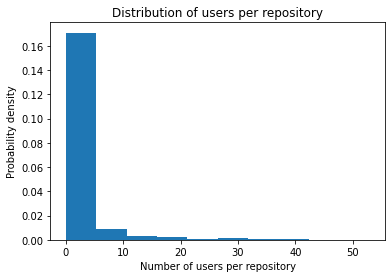
\includegraphics[scale=0.9]{user_repo_dist_hist.png}
    \caption{Hist diagram for the distribution of repositories per user}
    \label{fig:user_repo_dist_hist}
\end{figure}

\begin{figure}[H]
    \centering
    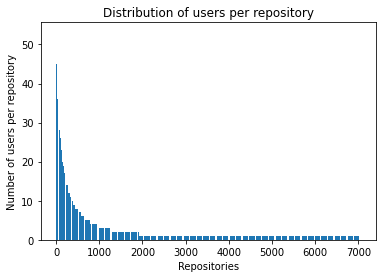
\includegraphics[scale=0.9]{user_repo_dist_bar.png}
    \caption{Bar diagram for the distribution of repositories per user}
    \label{fig:user_repo_dist_bar}
\end{figure}

\chapter{Methods}
\section{Knowledge graph construction}
\subsection{Nodes and edges selection}
This thesis constructed a heterogeneous graph to model the relationship between users and repositories by using Deep Graph Library \cite{wang2019dgl}. The nodes of the graph are users and repositories. There are 4 types of edges in the graph which are "watch", "star", "fork" and "own". "watch" means a user watches a repository. "star" means a user stars a repository. "fork" means a user forks a repository. "own" means a user is the owner of a repository. 

There are respectively 4 types of reverse relationships that are "watched-by", "starred-by", "forked-by" and "owned-by" between repositories and users. They are presented in the graph as the reverse edges for the aforementioned 4 types of edges. This is for the convenience of message passing and node aggregation during the training process.

Another research \cite{sun_personalized_2018} assigned the 4 types of edges with different scores in which the "watch" has the lowest score and the "own" has the highest score. This is a traditional rating based recommendation in which a high score is prefered and a lower one should be avoided. However, this thesis assigns those 4 types of edges with the same weight. Since any types of interactions between users and repositories should be interpreted as that a user is interested in a repository. It is different to the traditional recommendation in which a low score indicates that a user dislikes an item.

\subsection{Feature selection and presenting}
This thesis selected 3 features for users and 19 features for repositories. 

The 3 selected features of users are shown in the table \ref{tab:user_features}. The company was selected because the users from the same company may share the same interest. The location may help the neural network to recommend the repositories with the relevant natural languages. Users may write their hobbies and favourite programming languages in the 'bio' and a neural network thus can learn some hidden relationship between users.

\begin{center}
    \captionof{table}{The selected features of users}
    \begin{tabular}{| l | l |}
    \hline
    Feature & Description \\ \hline
    company & company name \\ \hline
    location & users' location \\ \hline
    bio & user's introduction \\ \hline
    \end{tabular}
    \label{tab:user_features}
\end{center}

The 18 features for repositories are shown in table \ref{tab:repo_features}. Some features may be empty for some repositories such as readme files, descriptions and so on. The empty feature will be presented as an empty string in the neural network.

\begin{center}
    \captionof{table}{The selected features of repositories}
    \begin{tabular}{| l | l |}
    \hline
    Feature & Description \\ \hline
    name & the name of a repository \\ \hline
    full\_name & repository's full name \\ \hline
    description & repository's description \\ \hline
    language & repository's programming language \\ \hline
    read\_me & repository's readme files \\ \hline
    source\_code & repository's source code \\ \hline
    license & repository's open source license \\ \hline
    size & the size of the repository \\ \hline
    stargazers\_count & number of stars of the repository \\ \hline
    watchers\_count & number of watches of the repository \\ \hline
    forks\_count & number of forks of the repository \\ \hline
    open\_issues & number of oppening issues of the repository \\ \hline
    subscribers\_count & number of subscribers of the repository \\ \hline
    has\_issues & whether the repository has issues or not \\ \hline
    has\_projects & whether the repository has projects or not \\ \hline
    has\_downloads & whether the repository has downloads available or not \\ \hline
    has\_wiki & whether the repository has wiki function enabled or not \\ \hline
    has\_pages & whether the repository has pages or not \\ \hline
    \end{tabular}
    \label{tab:repo_features}
\end{center}

Some features are strings that cannot be directly presented as inputs of the neural network. This thesis encoded them as vectors with the length of 50 bits by using a doc2vec model \cite{rehurek_lrec}. The vectors encoded by this model have an interesting property in which the vector distance of the strings with a similar meaning is close while the vector distance of strings with an opposite meaning is far away. This is helpful for the neural network to learn some potential relationships between repositories. The length of 50 bits is used because it is long enough to present the meaning of strings and not so robust for a neural network. All features are normalized. This is to prevent the neural network from biasing to some features with higher values.

Finally, the nodes, edges and normalized features are combined to form a heterogeneous graph.

\subsection{Training, validation and testing sub graphs}
The training, validation and testing subgraph were constructed from the aforementioned heterogeneous graph. This is to tune and test the neural network. The subgraphs were constructed through edge sampling with a ratio of 60:20:20 for training, validation and testing.

\subsection{Negative sampling}
To prevent the trained embeddings from folding, negative sampling is necessary. This thesis sampled negative edges of the same size as the positive edges. The negative training, validation and testing graph were constructed from those negative edges.

\subsection{Neural network design}
The neural network for the knowledge graph contains 3 layers which are the embedding layer, hidden layer and output layer. The embedding layer contains 2 sub single layer neural networks that are used to embedding users and repositories respectively. The hidden layer is a graph convolutional network (GCN) \cite{kipf_semi-supervised_2017} layer that contains 4 sub GCN layers for the 4 types of edges. The output of the 4 GCNs of the hidden layer will be aggregated with the sum aggregation. The output layer is also a GCN layer that contains 4 sub GCN layers. The output of the 4 GCNs of the output layer will also be aggregated with the sum aggregation. The output contains learned users representation and repositories representation.

Nodes in GCN will go through the process of message passing and aggregation with their neighbour nodes to get their new representation. In the process of message passing, every neighbour of a node sends its representation to the current node. In the process of aggregation, the current node aggregates the representation vectors received. The aggregation function has many types such as concatenate, sum and max. This thesis used sum aggregation. After the aggregation, the result will go through an activation function and calculate the new representation for the current node. The equation \ref{eq:message_passing_aggregation} depicts this process.

\begin{equation}
    h_u^{n+1}=\delta(sum(h_u^n, \sum_{v\in{N(u)}}h_v^n))
    \label{eq:message_passing_aggregation}
\end{equation}

The $h_u$ means the representation of the current node. The $\delta$ means the activation function. The $N(u)$ means the neighbour nodes of the current node. The $h_v$ means one of the neighbour nodes of the current node.

The learned representation vectors should be similar for nodes who have positive edges and dissimilar for those who have negative edges. The similarity is measured by their cosine similarity. The recommendation will be those with the highest similarity score.

\subsection{Loss function}
To make the neural network learn to output those representations, this thesis used a hinge loss function as shown in equation \ref{eq:loss_function}.

\begin{equation}
    l=\frac{1}{m\cdot{e}}\sum_{i=1}^{m}\sum_{j}^{e} max(0, f(n_u, n_v)+\Delta-f(p_u, p_v))
    \label{eq:loss_function}
\end{equation}

The $m$ means the number of types of edges (in this case it is 4). The $e$ means the number of edges. The $f$ means the cosine similarity. The $n_u$ and $n_v$ means the source and destination nodes for the negative edge $j$. The $p_u$ and $p_v$ means the source and destination nodes for the positive edge $j$. The $\Delta$ means the error tolerance.

\subsection{Training}

\subsection{Hyper parameters tuning}

\chapter{Baseline models}
\section{TF-IDF approach}
A TF-IDF approach proposed by \cite{sun_personalized_2018} was used as a baseline model for the evaluation of the KGNN based model. TF-IDF means term frequency and inverse document frequency which calculates the ratio between the frequency of the appearance of a term and the frequency of documents that contains the term. It can be used to measure the similarity between documents. The tf-idf vectors of documents with a similar topic tend to be similar.

This TF-IDF approach calculates the TF-IDF vectors for readme files and source code for all repositories. Then the 2 similarity matrices between repositories are carried out (one for the readme files and another one for the source code). The final similarity score between repositories is calculated by combining the 2 matrices using the equation \ref{eq:sim_repositories}. After the calculation of the similarity matrix, the algorithm recommends the most similar repositories to users.

\begin{gather}
    SIM(a,b)=\alpha\cdot{SIM_readme(a,b)}+\beta\cdot{SIM_src(a,b)}, \\
    s.t.\quad\alpha+\beta=1.
    \label{eq:sim_repositories}
\end{gather}

\section{Collaborate filtering approach}
A collaborative approach \cite{guendouz_recommending_2015} was also used as a baseline model for the evaluation of the KGNN based model. This approach measures the similarities between users and recommends the most "co-rated" repositories from the most similar users. The similarity measurement is the number of interactions (such as the number of stars).

% \subsection{Neural network based ranking model}

\section{Random recommendation}
Since traditional recommender systems suffer from data sparsity. They may end up in a poor performance during evaluation. To determine whether they work or not, this thesis used a random recommender as a contrast model. The poor performance models should be at least better than a random recommender model.

\chapter{Results and Discussion}
\section{Training results}
From the figure \ref{fig:training_results}, we can see that the hinge loss decreases sharply at the beginning and then stays stable at around 0.027.

\begin{figure}[H]
    \centering
    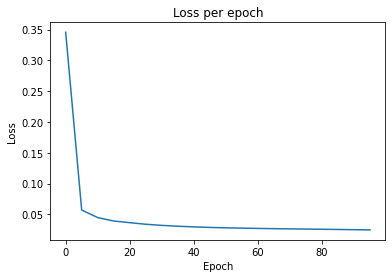
\includegraphics[scale=0.9]{training_results.png}
    \caption{The training results of the KGNN}
    \label{fig:training_results}
\end{figure}

\section{Metrics for the KGNN model}
\subsection{Hit rate}
According to the figure \ref{fig:hitrate_10}, the best overall hit rate for the top 10 is around 0.75 when the training epoch is 45. The epochs beyond 45 indicate that the neural network will be over-trained.

\begin{figure}[H]
    \centering
    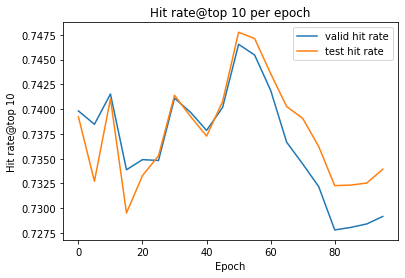
\includegraphics[scale=0.9]{hitrate@10.png}
    \caption{Hit rate@top 10 per epoch}
    \label{fig:hitrate_10}
\end{figure}

\subsection{Hit rate in different groups}
The users were split into 4 groups. The users in "group 0 to 5" have under 5 records of repository interactions(includes the star, watch, fork and own). Similarly, The users in "group 15 and above" have above 15 records of repositories.

According to the figure \ref{fig:hitrate_10_valid}, the hit rate for "group 15 and above" can reach 0.85 in the validation data set. The hit rate for "group 0 to 5" is stable and around 0.77. The hit rate for the middle tier (group 5 to 10 and 10 to 15) is quite poor compared with other tiers. The reason may be the number of records of the middle tier is small than that of the "group 0 to 5" which takes up about 80\% of the records. The reason why the "group 15 and above" has a high hit rate may be that the number of records of repositories is large and relatively easy to get hit.

The hit rate distribution \ref{fig:hitrate_10_test} of different groups for the testing data set is similar to that of the validation data set.

\begin{figure}[H]
    \centering
    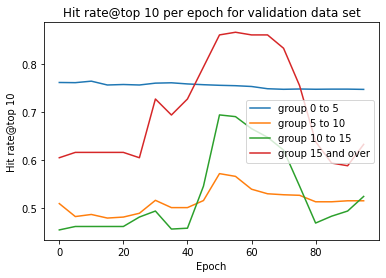
\includegraphics[scale=0.9]{hitrate@10_valid.png}
    \caption{Hit rate@top 10 per epoch for the validation data set}
    \label{fig:hitrate_10_valid}
\end{figure}

\begin{figure}[H]
    \centering
    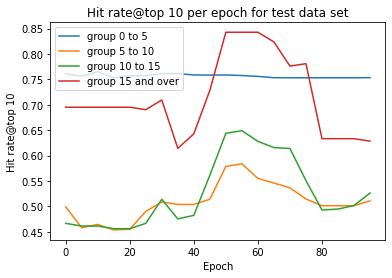
\includegraphics[scale=0.9]{hitrate@10_test.png}
    \caption{Hit rate@top 10 per epoch for the testing data set}
    \label{fig:hitrate_10_test}
\end{figure}

\subsection{AUC}
From the figure \ref{fig:auc}, the AUC score stays stable at around 0.7.

\begin{figure}[H]
    \centering
    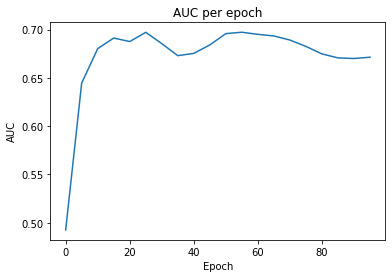
\includegraphics[scale=0.9]{auc.png}
    \caption{The AUC metric}
    \label{fig:auc}
\end{figure}

\section{Metrics for the TF-IDF approach}
\subsection{hit rate}
From the table \ref{tab:hitrate_10_tf-idf}, we can see that the performance is poor compared with the KGNN model.

\begin{center}
    \captionof{table}{Hit rate@top 10 for the TF-IDF approach}
    \begin{tabular}{| l | l | l | l | l | l |}
    \hline
    Top k & Overall & Group 0 to 5 & Group 5 to 10 & Group 10 to 15 & Group 15 to 20 \\ \hline
    10 & 0.042 & 0.039 & 0.040 & 0.073 & 0.106 \\ \hline
    \end{tabular}
    \label{tab:hitrate_10_tf-idf}
\end{center}

\section{Metrics for the collaborative filtering approach}
\subsection{hit rate}
From the table \ref{tab:hitrate_10_cf}, we can see that the performance is also poor compared with the KGNN model.

\begin{center}
    \captionof{table}{Hit rate@top 10 for the collaborative filtering approach}
    \begin{tabular}{l | l | l | l | l | l}
    \hline
    Top k & Overall & Group 0 to 5 & Group 5 to 10 & Group 10 to 15 & Group 15 to 20 \\
    \hline
    10 & 0.063 & 0.066 & 0.060 & 0.023 & 0.021 \\
    15 & 0.073 & 0.077 & 0.077 & 0.019 & 0.016 \\
    20 & 0.085 & 0.089 & 0.095 & 0.019 & 0.013 \\
    \end{tabular}
    \label{tab:hitrate_10_cf}
\end{center}

\section{Metrics for the random recommendation model}
From the table \ref{tab:hitrate_10_rand}, we can see that the performance of the random recommender is the poorest.

\begin{center}
    \captionof{table}{Hit rate@top 10 for the random recommender model}
    \begin{tabular}{| l | l | l | l | l | l |}
    \hline
    Top k & Overall & Group 0 to 5 & Group 5 to 10 & Group 10 to 15 & Group 15 to 20 \\ \hline
    10 & 0.001 & 0.001 & 0.000 & 0.000 & 0.007 \\ \hline
    15 & 0.002 & 0.002 & 0.000 & 0.002 & 0.006 \\ \hline
    20 & 0.004 & 0.004 & 0.006 & 0.003 & 0.006 \\ \hline
    \end{tabular}
    \label{tab:hitrate_10_rand}
\end{center}

\section{Discussion}
The performance of the KGNN model is the highest while other models have an extremely poor performance. The TF-IDF and collaborative filtering model are at least 10 times more accurate than the random recommender. It means that the TF-IDF and collaborative filtering model work but suffer from data sparsity. Based on this result, the KGNN model is promising in solving the data sparsity issues.

\subsection{RQ1}
Based on the experiment. The currently selected features include names, source code and readme files and so on. Some features have no impact on the performance such as "has\_wiki" and "has\_pages". Some features do play an important role in improving performance. Such as readme files and source code. If they are removed, the performance can drop significantly.

\subsection{RQ2}
The best overall performance for the KGNN model is 75\% hit rate@top 10 when the epoch is around 55.

\subsection{RQ3}
Compared with the baseline models. The performance is around 10 times better than that of baseline models in such a data set with high data sparsity.

\chapter{Conclusion}
Based on the results, the KGNN model can reduce the impact of data sparsity issues significantly. However, the performance is still not the best. Especially for the group 5 to 10 and 10 to 15 since they have fewer samples. Future work will explore the relationship between users (such as the following behaviour) to further improve the performance of the KGNN model in reducing the impact of data sparsity issues. The random walk and sampling techniques will also be integrated to enable the model to run on a larger scale.

% \appendix
% \chapter{Testbed Configuration}

\bibliographystyle{ieeetr}
\bibliography{Bib/strings,Bib/main}
\end{document}
